\documentclass[11pt]{article}
\usepackage{amsmath,amsbsy,amssymb,verbatim,fullpage,ifthen,graphicx,bm,amsfonts,amsthm}
\usepackage{graphicx}
\newcommand{\mfile}[1]  {{\small \verbatiminput{./#1}}} % Jeff Fessler, input matlab file
\newcommand{\tmop}[1]{\ensuremath{\operatorname{#1}}}
%\newcommand{\qed}{\hfill\ensuremath{\blacksquare}}
\newcommand{\R}{\mathbb{R}}
\newcommand{\C}{\mathbb{C}}
\newcommand{\Z}{\mathbb{Z}}
\newcommand{\A}{\mathcal{A}}
\newcommand{\minimize}{\operatorname*{minimize\ }}
\newcommand{\maximize}{\operatorname*{maximize}}
\newcommand{\st}{\operatorname*{\ subject\ to\ }}
\newcommand{\mtx}[1]{\mathbf{#1}}
\newcommand{\vct}[1]{\mathbf{#1}}
\def \lg       {\langle}
\def \rg       {\rangle}
\def \mA {\mtx{A}}
\def \mI {\mtx{I}}
\def \mU {\mtx{U}}
\def \mS {\mtx{S}}
\def \mV {\mtx{V}}
\def \mW {\mtx{W}}
\def \mLambda {\mtx{\Lambda}}
\def \mX {\mtx{X}}
\def \mY {\mtx{Y}}
\def \mZ {\mtx{Z}}
\def \zero     {\mathbf{0}}
\def \vzero    {\vct{0}}
\def \vone    {\vct{1}}
\def \vu {\vct{u}}
\def \vv {\vct{v}}
\def \vx {\vct{x}}
\def \vy {\vct{y}}
\def \vz {\vct{z}}
\def \vphi {\vct{\phi}}
\def \vmu {\vct{\mu}}
\def \R {\mathbb{R}}

\pagestyle{plain}

\title{{\bf Homework 1, CPSC 8420, Spring 2022}} % Change to the appropriate homework number
\author{\underline{Zhiyuan, Song}} % put your name in the LastName, FirstName format
\date{\today}

\begin{document}
\maketitle

\section*{Solution to Problem 1}
\begin{enumerate}
	\item {\bf Showing the Equivalence of two Ridge Regression Solutions:} 
	One can take SVD for an arbitary $\mA\in\R^{n\times p}$, $\mA=\mU\Sigma\mV$. $\mU\in\R^{n\times n}$ and $\mV\in\R^{p\times p}$ are complex unitary matrices.   .$\Sigma\in\R^{n\times p}$ is an rectangular diagonal matrix with non-negative real numbers on the diagonal. Concequently,
	\begin{gather*}
		\mA^{T}=\mV\Sigma\mU^{T}\\
		\mA^{T}\mA=\mV\Sigma\mU^{T}\mU\Sigma\mV^{T}=\mV\Sigma^{2}\mV^{T}\\
		\because \lambda\mI=\lambda\mV\mV^{T}=\mV\lambda\mV^{T}=\mV\lambda\mI\mV^{T}\\
		\therefore \mA^{T}\mA+\lambda\mI=\mV(\Sigma^{2}+\mI)\mV^{T}
	\end{gather*}
	\begin{align}\label{eqn:1:1}
	\therefore (\mA^{T}\mA+\lambda\mI)^{-1}\mA^{T}=\mV\Sigma(\Sigma^{2}+\lambda\mI)^{-1}\mU^{T}
	\end{align}
	On the other hand,
	\begin{gather*}
	\mA\mA^{T}=\mU\Sigma^{2}\mU^{T}\\
	\because \lambda\mI=\lambda\mU\mU^{T}=\mU\lambda\mU^{T}=\mU\lambda\mI\mU^{T}\\
	\therefore \mA\mA^{T}+\lambda\mI=\mU(\Sigma^{2}+\lambda\mI)\mU
	\end{gather*}
	\begin{align}\label{eqn:1:2}
	\therefore \mA^{T}(\mA\mA^{T}+\lambda\mI)^{-1}=\mV\Sigma(\Sigma^{2}+\lambda\mI)^{-1}\mU^{T}
	\end{align}
	We can observe that eq\ref{eqn:1:2} is equivalent to 	eq\ref{eqn:1:1}.
	\item {\bf Time Consumption for Different $p$ of $\mA$:} Matrix $\mA\in\R^{100\times p}$ with random elements was introduced for a certein $p$. $\beta$ were computed using two equivalent solutions of ridge regression and the time for each execuation was recorded, as shown in Figure \ref{fig:p1}.
	\begin{figure} % This is how figure are placed into latex document
		\centering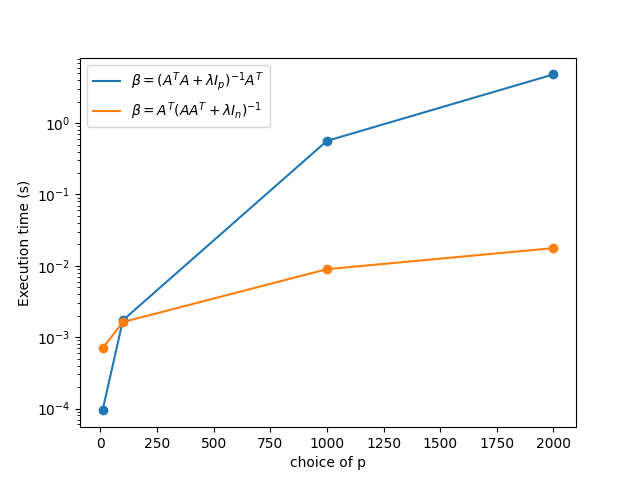
\includegraphics[width=.75\linewidth]{p1.png}
	 	\caption{Time consumption for various $p$ of $\mA$.} % caption of the figure
	 	\label{fig:p1}  % Label the figure so you can refer to it in text.
	\end{figure}
\end{enumerate}
\section*{Solution to Problem 2}
\begin{enumerate}
	\item {\bf Error Equation Dervation:}
	\begin{align*}
	Err(x_{0}) & = E\left[(Y-\hat{f}(x_{0}))^{2}|X=x_{0}\right]\\
	& = E\left[(Y-f(x_{0})+f(x_{0}-\hat{f}(x_{0})))^{2}\right]\\
	& = E\left[(Y-f(x_{0}))^{2}+(f(x_{0})-\hat{f}(x_{0}))^{2}+2(Y-f(x_{0}))(f(x_{0})-\hat{f}(x_{0}))\right]\\
	& = \sigma^{2}+E\left[(f(x_{0})+E[\hat{f}(x_{0})\right]-E\left[\hat{f}(x_{0})]-\hat{f}(x_{0}))^{2}\right]+2E\left[(Y-f(x_{0}))(f(x_{0})-\hat{f}(x_{0}))\right]
	\end{align*}
	Where $2E[(Y-f(x_{0}))(f(x_{0})-\hat{f}(x_{0})) = 0$ because $E(\epsilon)=0$. Meanwhile, $E[(Y-f(x_0))^2]=E[\epsilon^2]=Var(\epsilon)+E^{2}[\epsilon]=\sigma^2$. Therefore,
	\begin{align*}
	Err(x_{0}) = \sigma^{2}+E\left[(f(x_{0})-E[\hat{f}(x_{0})])^{2}\right]+E\left[(\hat{f}(x_{0})-\hat{f}(x_{0}))^{2}\right]\\
	+2E\left[(f(x_{0})-E[\hat{f}(x_{0})])(E[\hat{f}(x_{0})]-\hat{f}(x_{0}))\right]\\
	= \sigma^{2}+E\left[(f(x_{0})-E[\hat{f}(x_{0})])^{2}\right]+E\left[(\hat{f}(x_{0})-\hat{f}(x_{0}))^{2}\right]\\
	+2(f(x_{0})-E[\hat{f}(x_{0})])E\left[(E[\hat{f}(x_{0})]-\hat{f}(x_{0}))\right]
	\end{align*}
	Because $E\left[E[\hat{f}(x_{0})]-\hat{f}(x_{0})\right]=0$, leading to 0 cross term. Consequently,
	\begin{align*}
	Err(x_{0})& = \sigma^{2}+E\left[(f(x_{0})-E[\hat{f}(x_{0})])^{2}\right]+E\left[(E[\hat{f}(x_{0})]-\hat{f}(x_{0}))^{2}\right]\\
	& = \sigma^{2}+(f(x_{0})-E[\hat{f}(x_{0})])^{2}+E\left[(E[\hat{f}(x_{0})]-\hat{f}(x_{0}))^{2}\right]\\
	& = \sigma^{2}+Bias(\hat{f}(x_{0}))^{2}+Var(\hat{f}(x_{0}))
	\end{align*}
	In the case of $k$-NN, the expectation term, $E[\hat{f}(x_0)]$, can be evalueated
	\begin{align*}
	E[\hat{f}(x_0)] & = E\left[\frac{1}{k}\sum_{l=1}^{k}Y_l\right]\\
	& = E\left[\frac{1}{k}\sum_{l=1}^{l}(f(x_l)+\epsilon_l)\right]\\
	& = \frac{1}{k}\sum_{l=1}^{k}(f(x_l)+\frac{1}{k}\sum_{l=1}^{k}E[\epsilon_l])\\
	& = \frac{1}{k}\sum_{l=1}^{k}(f(x_l)
	\end{align*}
	Next, we can simplify the bias term using the evaluation of the expectation.
	\begin{align*}
	Bias^{2}(x_0) & = (f(x_0)-E[\hat{f}(x_0)])^2\\
	& = \left(f(x_0)-\frac{1}{k}\sum_{l=1}^{k}f(x_l)\right)^2
	\end{align*}
	The variance of $k$-NN can be simplified
	\begin{align*}
	Var(\hat{f}(x_0)) & = E\left[\left(\hat{f}(x_0)-E[\hat{f}(x_0)]\right)^2\right]\\
	& = E\left[\left(\frac{1}{k}\sum_{l=1}^{k}Y_l - \frac{1}{k}\sum_{l=1}^{k}f(x_l)\right) \right]\\
	& = E\left[\left(\frac{1}{k}\sum_{l=1}^{k}(f(x_l)+\epsilon_l) - \frac{1}{k}\sum_{l=1}^{k}f(x_l)\right) \right]\\
	& = \frac{1}{k^2}E\left[ \left(\sum_{l=1}^{k}\epsilon_l \right)^2\right]\\
	& = \frac{1}{k^2}Var\left(\sum_{l=1}^{k}\epsilon_l\right)
	\end{align*}
	Because $Var\left(\sum_{l=1}^{k}\epsilon_l\right)=E\left[\left(\sum_{l=1}^{k}\epsilon_l-E\left[\sum_{l=1}^{k}\epsilon_l\right]\right)^2\right]$ and $E\left[\sum_{l=1}^{k}\epsilon_l\right]=\sum_{l=1}^{k}E[\epsilon_l]=0$. Accordingly, we can obtain the variance term
	\begin{align*}
	Var(\hat{f}(x_0))&=\frac{1}{k^2}\sum_{l=1}^{k}Var(\epsilon_l)\\
	& = \frac{k\sigma^2}{k^2}=\frac{\sigma^2}{k}
	\end{align*}
	As a result, we can combine Bias term and Variance term together, one can obtain error formula in the case of $k$-NN
	\begin{align*}
	Err(x_0) = \sigma^{2}+[f(x_{0})-\frac{1}{k}\sum_{l=1}^{k}f(x_{l})]^{2}+\frac{\sigma^{2}}{k}
	\end{align*}
	\item {\bf Justification of Bias and Variance change when $k$ increases:} The number of neighbors $k$ is inversely related to the model complexity. For small $k$, the estimate $\hat{f}_{k}(x)$ can potentially adapt itself better to the underlying $f(x)$. When k increases, the the squared difference between $f(x_{0})$ and the average of $f(x)$ at the k-nearest neighbors (i.e., the bias) will typically increase and the mean of the data set includes less and less information. While the variance will decrease according to its role in the variance term.
\end{enumerate}
\section*{Solution to Problem 3}
{\bf For vanilla linear regression model:}
\begin{align*}
	\hat{\bm{\beta}}_{LS}=\min_{\bm{\beta}} \|\vy-\mA\bm{\beta}\|_2^2 \\
	\nabla\|\mA\bm{\beta}-\vy\|^{2}_2=2\mA^{T}(\mA\bm{\beta}- \vy)
\end{align*}
Let $\nabla \|\mA\bm{\beta}-\vy \|^{2}_2=0$, one can obtain
\begin{align*}
	\mA^{T}\mA\bm{\beta}=\mA^{T}\vy
\end{align*}
Therefore,
\begin{align}\label{eqn:3:1}
	\hat{\bm{\beta}}_{LS}=(\mA^{T}\mA)^{-1}\mA^{T}\vy=\mA^T\vy
\end{align}
{\bf For ridge regression model:} 
\begin{align*}
\hat{\bm{\beta}}_{\lambda}^{Ridge}=\min_{\bm{\beta}}\|\mA\bm{\beta}-\vy\|^2_2+\lambda\|\bm{\beta}\|^2_2\\
\nabla(\|\mA\bm{\beta}-\vy\|^2_2+\lambda\bm{\beta})=2\mA^{T}(\mA\bm{\beta}-\vy)+2\lambda\bm{\beta}
\end{align*}
Applying same method, one can get
\begin{align*}
	\mA^T(\mA\bm{\beta}-\vy)+\lambda\bm{\beta}=0
\end{align*}
Accordingly,
\begin{align}\label{eqn:3:2}
	\hat{\bm{\beta}}_{\lambda}^{Ridge}=(\mA^{T}\mA+\lambda\mI)^{-1}\mA^{T}=\frac{A^{T}\vy}{1+\lambda}=\frac{\hat{\bm{\beta}}_{LS}}{1+\lambda}
\end{align}
{\bf For Lasso model:}
\begin{align*}
	\hat{\bm{\beta}}_\lambda^{Lasso} =\min_{\bm{\beta}} \frac{1}{2}\|\vy-\mA\bm{\beta}\|_2^2+\lambda \|\bm{\beta}\|_1
\end{align*}
We know that, if function $f$ and $g$ are both concex functions, $f+g$ must be convex. Hence, Lasso model must have a globla minimium theoretically. As for function, $f(x)=|x|$, it is not defferatiable at $x=0$. However, if sub-defferentials is introduced, one can get modified differentials for $f(x)=|x|$ at $x=0$, $\delta f(x)=\text{sign}(x)$. $\text{sign}(x)$ is defined as,
\begin{align}\label{eqn:3:3}
	\text{sign}(x)=
	\begin{cases}
	-1 & \text{if } x<0\\
	[-1,1] & \text{if } x=0\\
	1 & \text{if } x>0
	\end{cases}
\end{align}
With the complement of the defferential at $x=0$, we can take derivative for Lasso model to obatin the minimization by making the defferential term equal to 0.
\begin{align*}
	\nabla \frac{1}{2}\|\mA\bm{\beta}-\vy\|^2_2+\delta\lambda\|\bm{\beta}\|_1=0\\
	\therefore \mA^{T}(\mA\bm{\beta}-\vy)+\lambda \text{ sign}(\bm{\beta})=0
\end{align*}
Note that $\mA^{T}\mA=\mI$, we can obtain
\begin{align*}
	\hat{\bm{\beta}}^{Lasso}_\lambda=\mA^T\vy-\lambda \text{ sign}(\hat{\bm{\beta}}^{Lasso}_\lambda)
\end{align*}
we can notice that $\mA^T\vy$ is the solution of $\hat{\bm{\beta}}_{LS}$.Accordingly, we can keep writing the expression
\begin{align}\label{eq:3:4}
	\hat{\bm{\beta}}^{Lasso}_\lambda=
	\begin{cases}
	\hat{\bm{\beta}}_{LS}+\lambda & \text{if } \hat{\bm{\beta}}_{LS} < -\lambda\\
	0 & \text{if } |\hat{\bm{\beta}}_{LS}| \leq \lambda\\
	\hat{\bm{\beta}}_{LS}-\lambda & \text{if } \hat{\bm{\beta}}_{LS} > \lambda\\
	\end{cases}=\text{sign}(\hat{\bm{\beta}}_{LS})(|\hat{\bm{\beta}}_{LS}|-\lambda)_+
\end{align}
The equation above is recognized as a soft-thresholding function defined as
\begin{align*}
\mathbb{S}_{\lambda}(x)=
\begin{cases}
x+\lambda & \text{if } x<-\lambda\\
0 & \text{if } |x|\leq\lambda\\
x-\lambda & \text{if } x>\lambda\\
\end{cases}
\end{align*}
Therefore, we can denote the solution for Lasso model as
\begin{align}\label{eq:3:5}
\hat{\bm{\beta}}^{Lasso}_\lambda=\mathbb{S}_{\lambda}(\hat{\bm{\beta}}_{LS})
\end{align}
{\bf For subset selection model:}
We can solve the subset model using
\begin{align*}
	\min_{\bm{\beta}} \frac{1}{2} \|\vy-\mA\bm{\beta}\|_2^2 + 
	\lambda\|\bm{\beta}\|_0
\end{align*}
It is equivalent to solve non-convex problem
\begin{align*}
\min_{\bm{\beta}} \frac{1}{2} \|\vy-\mA\bm{\beta}\|_2^2 \st & \ \|\bm{\beta}\|_0 \leq k
\end{align*}
Where the $l_0$ norm of a vector $\bm{\beta}$ counts the number of non zero results in $\bm{\beta}$ and is given by $\|\bm{\beta}\|_0=\sum_{i=1}^{p}1(\bm{\beta\neq 0})$. According to the definition of subset selection model, the solution can be expressed
\begin{align}
	\hat{\bm{\beta}}_{\lambda}^{Subset}=\hat{\bm{\beta}}_{LS}I(|\hat{\bm{\beta}}_{LS}|\geq|\hat{\bm{\beta}}_{(M)}|)
\end{align}
For those coefficients less than the $\text{M}^{\text{th}}$ largest coefficient will be set to 0.
\section*{Solution to Problem 4}
\begin{enumerate}
	\item {\bf Loading and shuffling data from house.data}
	The code starts from importing useful global packages to perform array calculations, standardization and linear regressions. The functions of linear regression, ridge regression and mean of square error were defined beforehand. Data shuffling was performed and the seed (seed = 2023) was provided for checking. Data splitting and standardization will be taken in the coming sub problems.
	\mfile{prob4-1.txt}
	\item {\bf Mean squared error as a function of training set}
	\begin{figure}
		\centering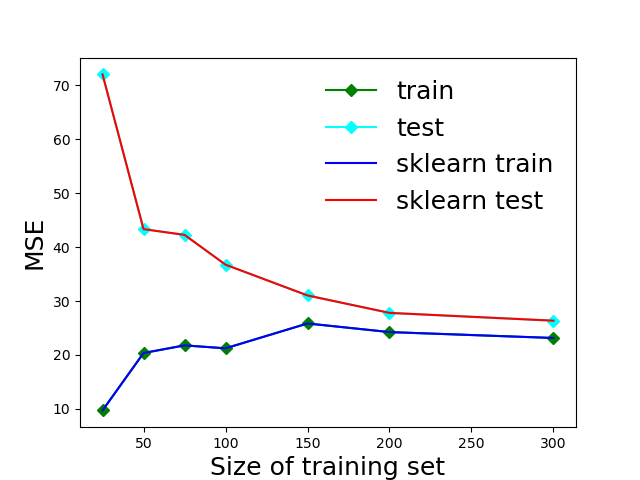
\includegraphics[width=.75\linewidth]{4_2_fig.png}
		\caption{MSE for training and test data as a function of training set size} % caption of the figure
		\label{fig:p4-2}  % Label the figure so you can refer to it in text.
	\end{figure}
	Data was standardized using zscore after splitting for each training set and test set. Linear regression, which maximize least square error, were performed for training set. The result of MSE calculations between test set of output and predicted output using trained coefficients was demonstrated in Figure \ref{fig:p4-2}. Herein, the linear regression was defined as a function using matrix computations and examined by build-in python package, sklearn. We can see results from both methods coincided in the case of either training or test, meaning the same predictions they were able to get and validating the self-built function. As more training data was included, the MSE of the training MSE grew slower due to better fittings but more errors introduced. Whereas the predictions became more accurate and the test set size was reduced, leading to a decrease of MSE for the set. The two curves will eventually meet because the training curve is typically increasing while test MSE is decreasing.
	\mfile{prob4-2.txt}
	\item {\bf MSE vs Degree expansion} Similar treatments and global packages were applied before the degree expansion. The feature set was expanded every time when the order of magnitude of the original features increases. The expanded features were standardized before they incorporated with the data previously treated. Because there is a feature of house prising containing either 0 or 1, the degree extension of the data set results in the same data set, causing an invertable $\mA^{A}A$. Hence, we need to apply pseudoinverse for the inversion of $\mA^{A}A$ (pinv() instead of inv() used in the code). The result of self-built function was examined by calling python sklearn package, as shown in Figure \ref{fig:p4-3}. And we can observe a slight decrease at degree 2 for test set, indicating the degree extension of 2 can offer the best prediction in terms of MSE. While, MSE of training set kept reducing as higher degree features were involved, which resulted in an overfitting. Hence, such an overfitting caused the steep increase of the test set MSE as the degree increased.
	\begin{figure}
		\centering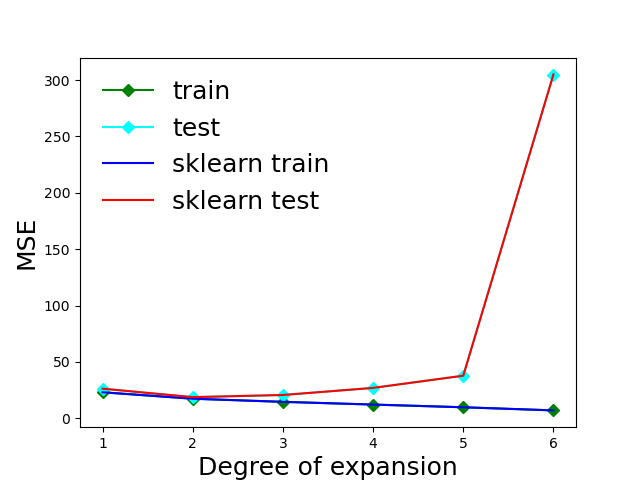
\includegraphics[width=.75\linewidth]{4_3_fig.png}
		\caption{MSE for training and test data as a function of expansion degree} % caption of the figure
		\label{fig:p4-3}  % Label the figure so you can refer to it in text.
	\end{figure}
	\mfile{prob4-3.txt}
	\item {\bf MSE vs Ridge Regression}
	The solution of ridge regression will approach that of the conventional regression if $\lambda$ is extremely small. Therefore, we should observe a similar big gap between training and test curves with 6-degree extension (Figure \ref{fig:p4-3}) when $\lambda$ is significantly small. The result of self-built function was examined by calling python sklearn package, as shown in Figure \ref{fig:p4-4}. Pseudo-inverse was also applied here as a results of degree extension. Besides, the offset was considered due to the standardized input but the original output, leading to the identity of $p+1$ dimension in the ridge regression. However, the intercept term keeps constant. Therefore, the $\lambda$ was only allowed to multiply the remaining $p\times p$ identity and leave the first term as shown in the code. As $\lambda$ increases, it starts to regulate the variance and force the minimization involving the $\|\bm{\beta}\|^2_2$ term, avoiding overfitting and leading to a drop of test MSE. However, some significant coefficients will become very small if $\lambda$ becomes too large, causing an increase of the bais. Accordingly, it will lead to an increase of MSE. AS for training set, overfitting problem will be regulated but some coefficients' decreases lead to larger variance, causing the increase of its MSE.
	\begin{figure}
		\centering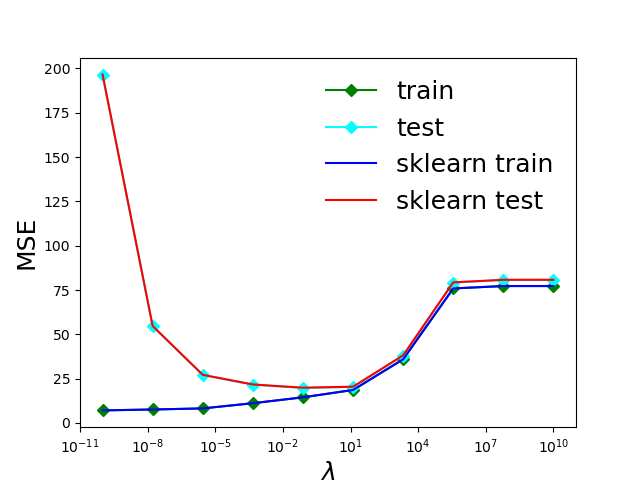
\includegraphics[width=.75\linewidth]{4_4_fig.png}
		\caption{MSE for training and test data as a function of $\lambda$ in ridge regression} % caption of the figure
		\label{fig:p4-4}  % Label the figure so you can refer to it in text.
	\end{figure}
	\mfile{prob4-4.txt}
	\item {\bf coefficients vs $\lambda$ in Lasso regression}
	To show a better variation for coefficients, the range for $\lambda$ was set from $10^{-4}$ to $10^2$. The solution of the ridge regression will approach the result of the conventional regression if $\lambda$ is significantly small. However, some coefficients become zero as the $\lambda$ increases, indicating the corresponding features hardly contribute to the output. All coefficients will reach zero if $\lambda$ increases. It l results in a trivial solution finally that contains nothing but the intercept, $\bm{\beta}_0$, as shown in Figure \ref{fig:p4-5}.
	\mfile{prob4-5.txt}
	\begin{figure}
		\centering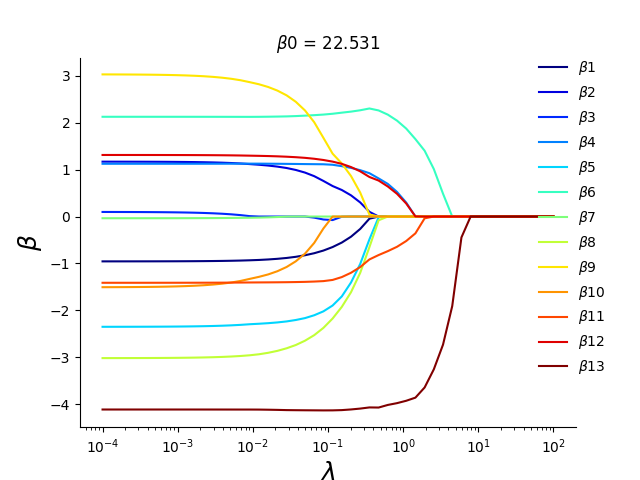
\includegraphics[width=.75\linewidth]{4_5_fig.png}
		\caption{$\bm{\beta}$ as a function of $\lambda$ in Lasso regression} % caption of the figure
		\label{fig:p4-5}  % Label the figure so you can refer to it in text.
	\end{figure}
\end{enumerate}
\end{document}
